\documentclass[12pt]{article}
\setlength\parindent{0pt}
\usepackage{fullpage}
%\usepackage[margin=0.5in, paperwidth=13.5in, paperheight=8.4375in]{geometry}
\usepackage[margin=0.5in, paperwidth=8.5in, paperheight=11in]{geometry}

\usepackage{amsmath}
\usepackage{graphicx}
\newcommand{\BI}{\begin{itemize}}
\newcommand{\insp}{\vspace{1in}}
\newcommand{\EI}{\end{itemize}}
\newcommand{\BE}{\begin{enumerate}}
\newcommand{\EE}{\end{enumerate}}
\newcommand{\BS}{\bigskip}
\setlength{\parskip}{4mm}


\pagenumbering{gobble}

\begin{document}

\begin{center}
	\Large \sc Homework Quiz 1 - Stellar Motion
\end{center}

\begin{flushright}
	Name: \underline{\hspace{4in}}
\end{flushright}

\it Instructions: Answer the question on the front and the two questions on the back. 

\rm
	
	\begin{enumerate}
		\item Someone in Syracuse sees a star directly east of Polaris at 9 PM, as shown on the diagram as a red starburst.  The position of Polaris in Syracuse is also shown{\it Note that these diagrams have the east/west typo corrected, so you don't need to do that.} 
		
		\begin{center}
		\begin{minipage}{0.45\textwidth}
			\begin{center}
\it Sky Above Horizon\\
				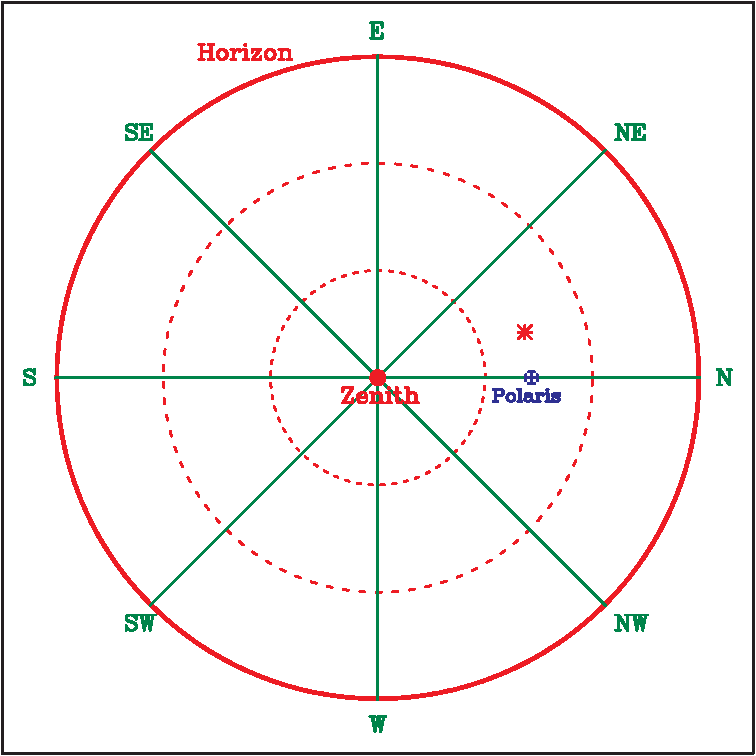
\includegraphics[width=0.9\textwidth]{quiz-1-crop.pdf}
			\end{center}
		\end{minipage}
		\begin{minipage}{0.45\textwidth}
			\begin{center}
				\it Sky Below Horizon\\
				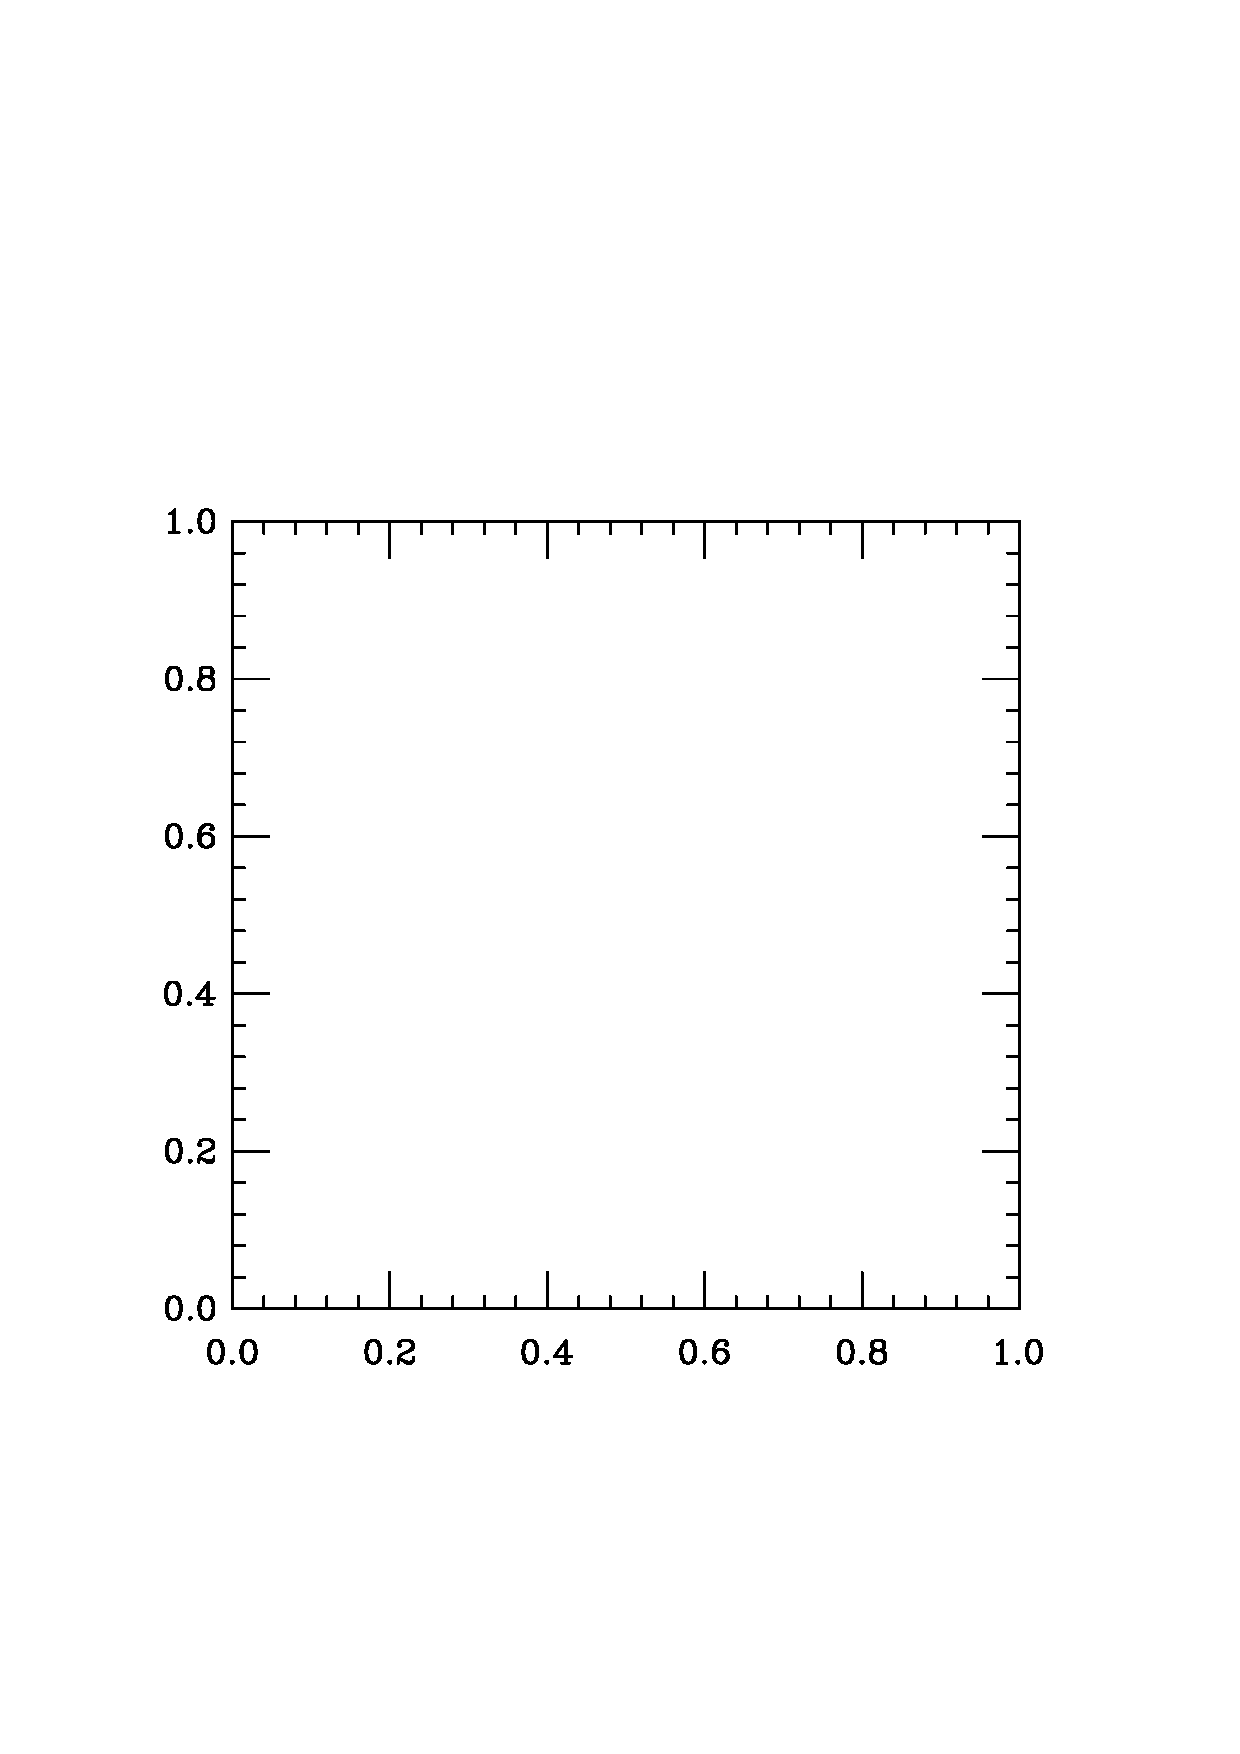
\includegraphics[width=0.9\textwidth]{botsky-crop.pdf}
			\end{center}
		\end{minipage}
		\end{center}
		
		Draw the path of that star. Then label its position at 3 AM.
		
		\newpage
		
		\item Where would an observer in Rio de Janeiro, Brazil (latitude $23^\circ S$) find the North Celestial Pole? Where would they find the South Celestial Pole? {\it (You may describe clearly in words and/or label on the diagrams.)}
		
				\begin{center}
			\begin{minipage}{0.4\textwidth}
				\begin{center}
					\it Sky Above Horizon\\
					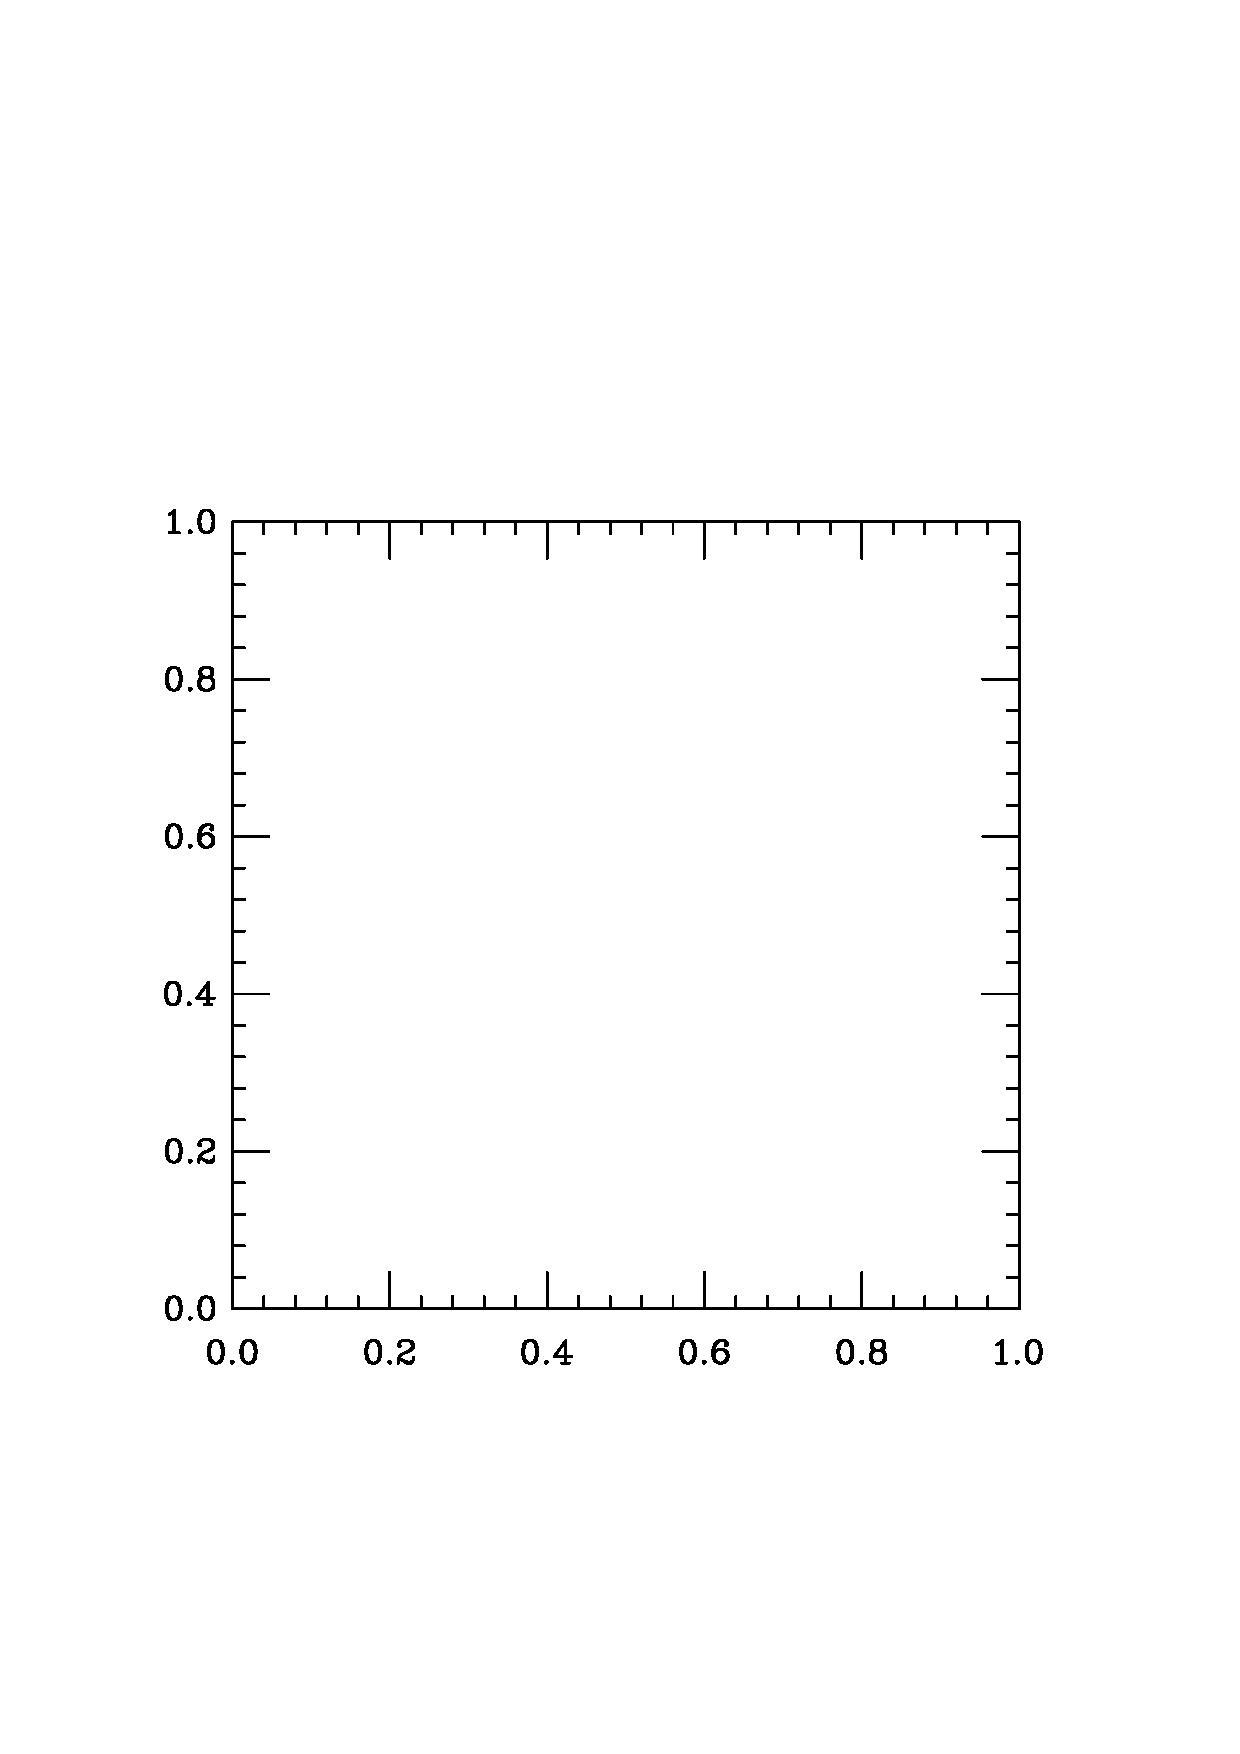
\includegraphics[width=0.8\textwidth]{topsky-crop.pdf}
				\end{center}
			\end{minipage}
			\begin{minipage}{0.4\textwidth}
				\begin{center}
					\it Sky Below Horizon\\
					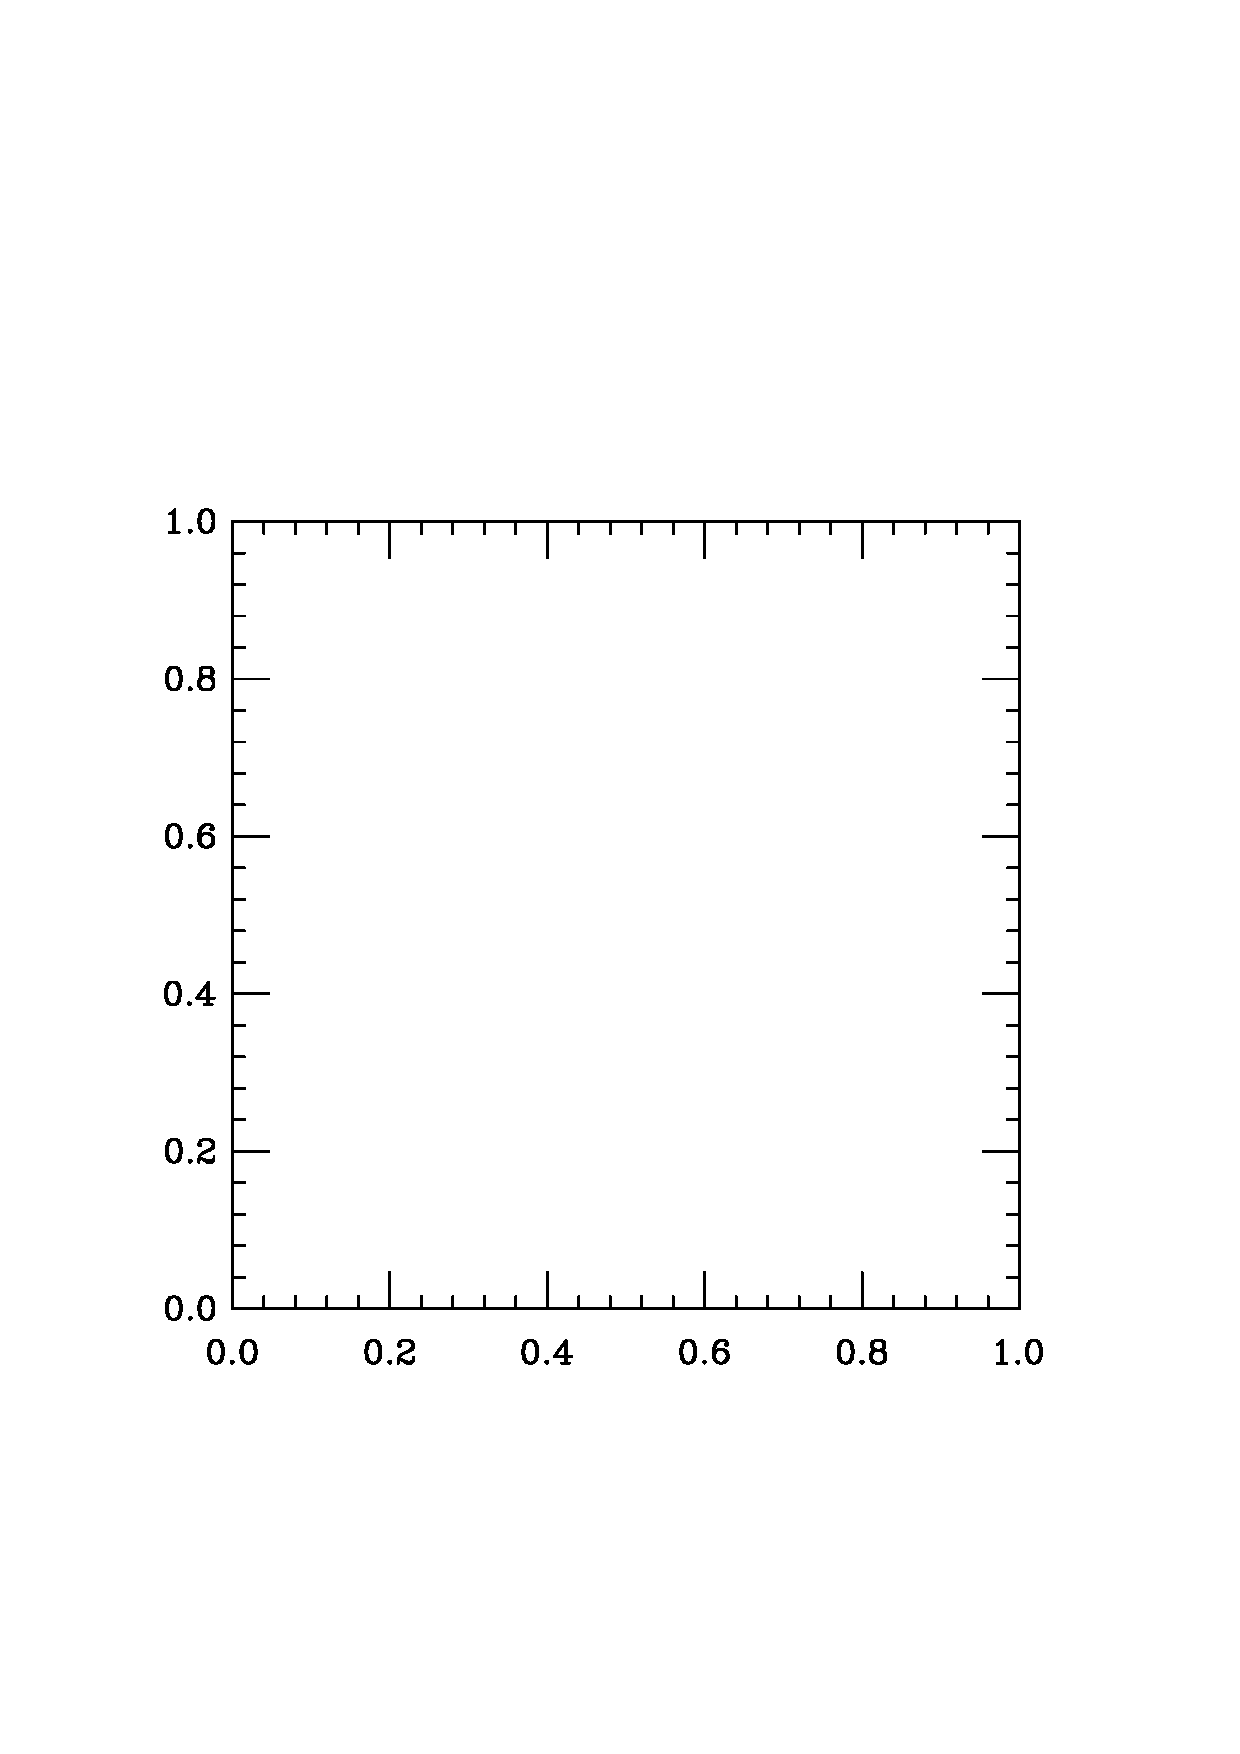
\includegraphics[width=0.8\textwidth]{botsky-crop.pdf}
				\end{center}
			\end{minipage}
		\end{center}
		
		
		\vspace{1.5in}
		
		\item As seen from Syracuse (latitude $43^\circ S$), the star Deneb is almost always in the sky; it dips below the northern horizon for only a few hours each day.
		
		How would someone in Reykjavik, Iceland (latitude $64^\circ N$) see Deneb move? Draw its path on the diagrams below. 
		
						\begin{center}
			\begin{minipage}{0.4\textwidth}
				\begin{center}
					\it Sky Above Horizon\\
					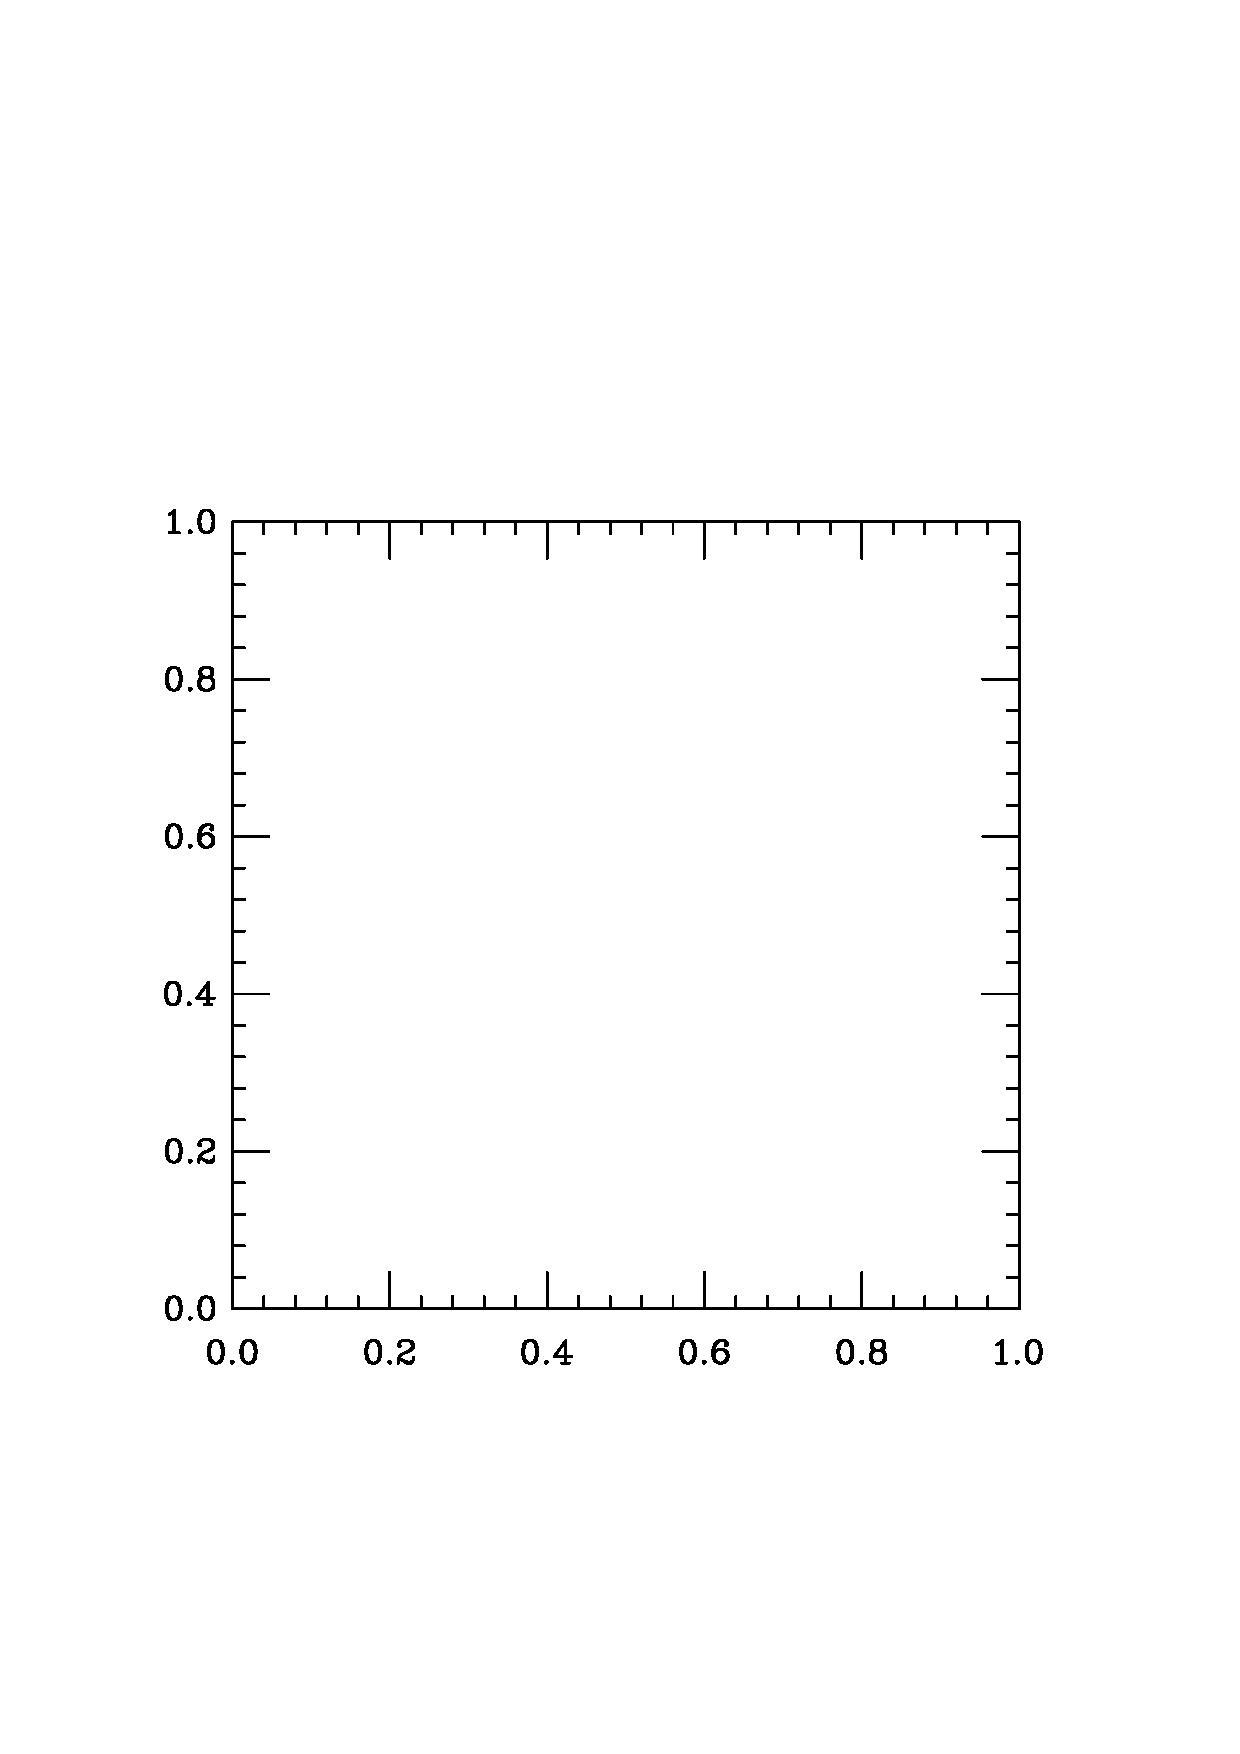
\includegraphics[width=0.8\textwidth]{topsky-crop.pdf}
				\end{center}
			\end{minipage}
			\begin{minipage}{0.4\textwidth}
				\begin{center}
					\it Sky Below Horizon\\
					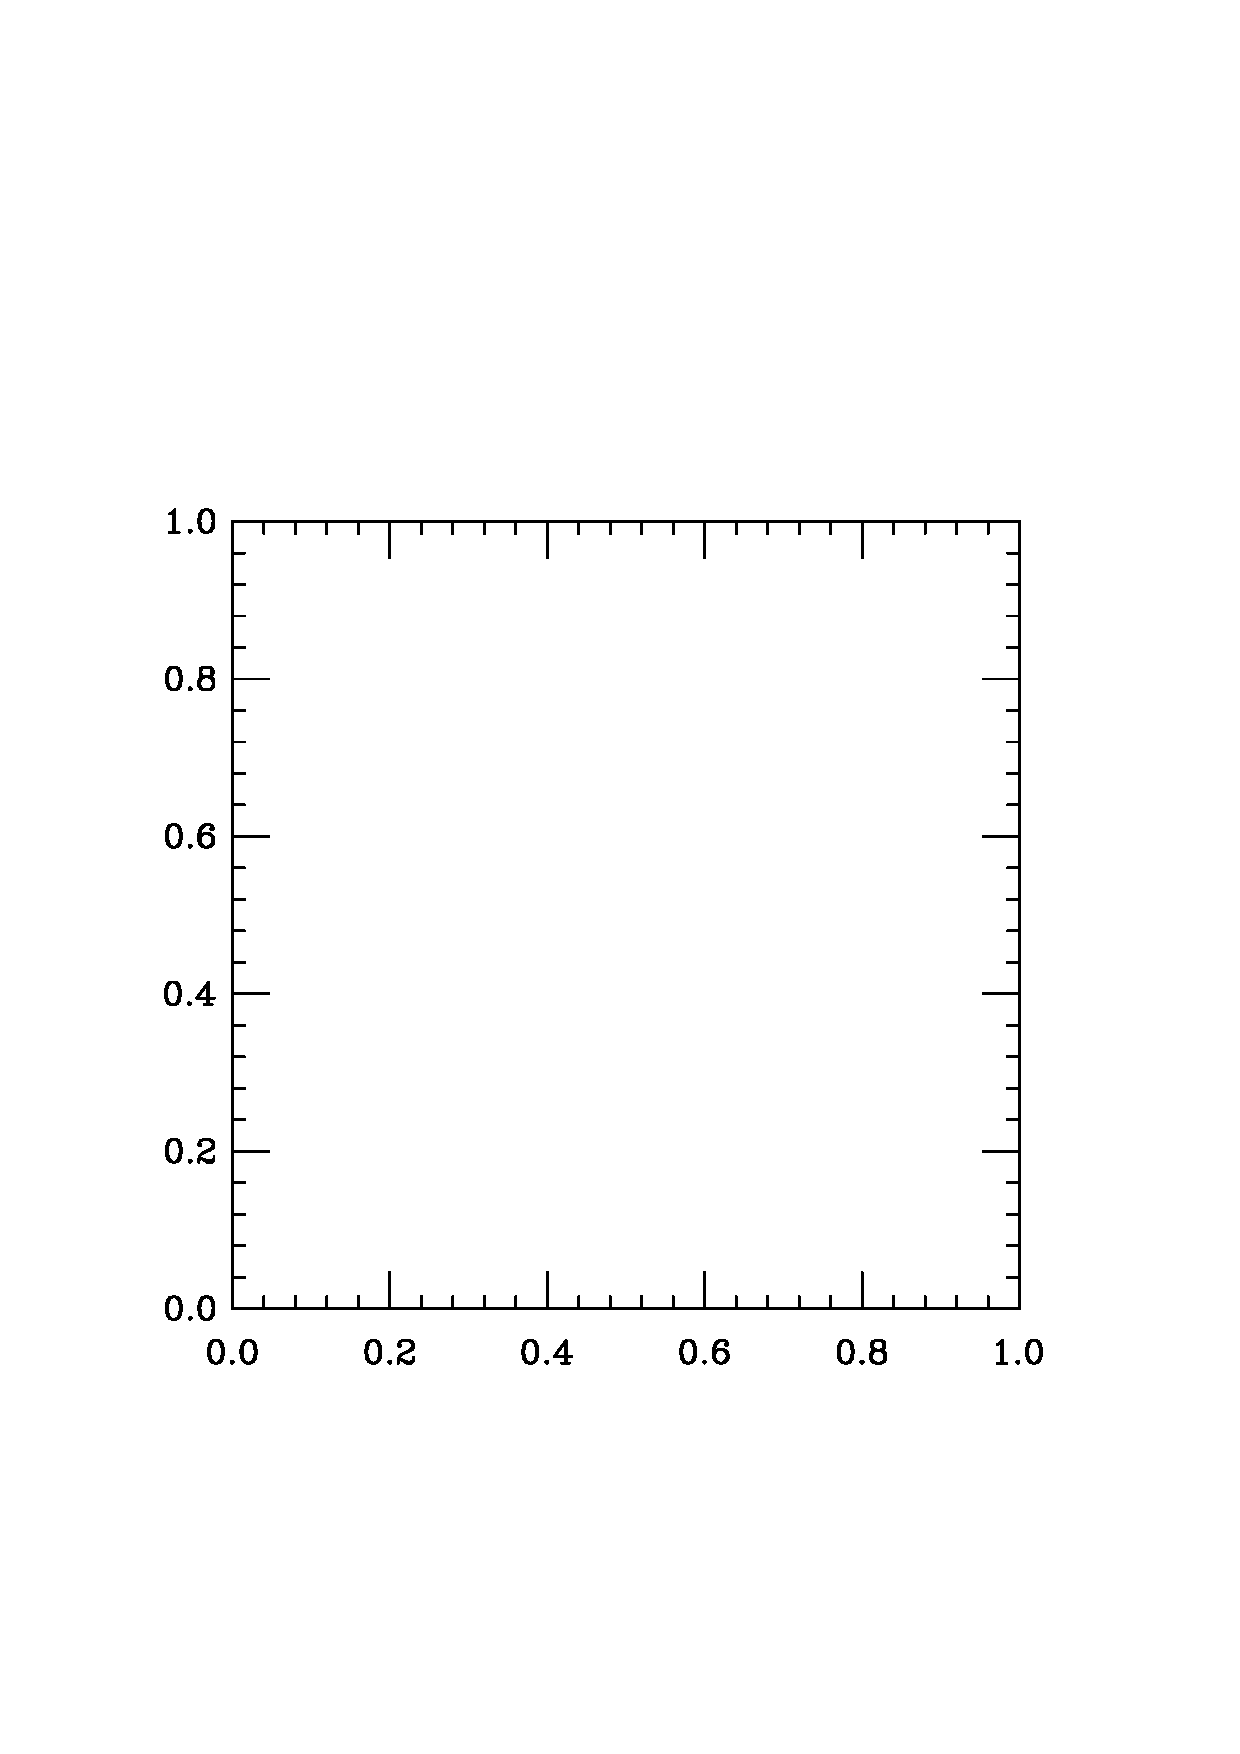
\includegraphics[width=0.8\textwidth]{botsky-crop.pdf}
				\end{center}
			\end{minipage}
		\end{center}
		
	\end{enumerate}
	
	
		
		
		
	
\end{document}
	
	
	
	